% !TeX root=../main.tex%
\chapter{ نتیجه گیری و پیشنهاد ها}
\section{
نتیجه گیری
}
پروژه حاضر یک شیوه برای مدل کردن مدار های الکتریکی و حل آن به صورت خودکار ارائه میدهد؛
همانطور که پیش تر اشاره شد تمرکز این پژوهش بر ایجاد یک کتابخانه پایتون بوده و هدف ایجاد یک اپلیکیشن مانند
\lr{spice}
و بررسی آن از زاویه مهندسی نرم افزار نیست.
\section{
	پژوهش های مشابه
}
شاید بتوان کتابخانه
\lr{pyspice}
را شبیه ترین پژوهش به پژوهش حاضر نامید،
که امکانات زیادی را در اختیار برنامه نویسان برای حل مدار های الکتریکی قرار میدهد؛
ولی تفاوت اصلی آن با این پروژه این است که
\lr{pyspice}
مسائل را با آنالیز ها و مدل های متفاوتی انجام میدهد ولی در این پژوهش همه مسائل توسط یک مدل واحد حل میشود؛ بدین معنی که مفهوم مدار به عنوان یک گراف در نظر گرفته شده است.
\footnote{
	نام این پروژه از همین موضوع گرفته شده است؛
	\lr{gracc}
	یا همان
	\lr{graph of circuit}
}

\section{پیشنهاد برای ادامه پژوهش}
همانطور که پیشتر در قسمت
\ref{section:atm}
توضیح داده شد،
 این پروژه از توصیف متنی برای مدار ها استفاده میکند. ولی اگر مدلی طراحی کنیم که مدار را به صورت عکس از کاربر گرفته و آن را به توصیف متنی مدار تبدیل کند آنگاه میتوان با استفاده از ساختار شکل 
 زیر با داشتن عکس مدار جواب آن را یافت!
 البته تلاش هایی در این زمینه شده که از طریق این
 \href{https://github.com/Mehrdadghassabi/Hand-Drawn-Circuits}{پیوند} 
  قابل دسترسی است.
  
\begin{figure}[ht]
	\centerline{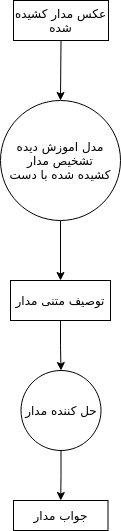
\includegraphics[width=3cm]{fig9}}
	\caption{ساختار جواب دادن به مدار کشیده شده به صورت دستی
	}
\end{figure}
